\section{DEM study: effective conductivity with disrupted packing}
\label{sec:dem-studies-effective-conductivity}

\subsection{Model Setup \& Methodology}\label{sec:dem-setup}
We analyze a three-dimensional pebble bed consisting of mono-dispersed particles of diameter $d_p$. The particles are constrained by rigid $y-z$-planes at locations of $\frac{x}{d_p} = \pm 10$ (the walls of our container). There are periodic boundary conditions in the $y$-direction located at $\frac{y}{d_p} = \pm 7.5$. Gravity acts in the negative $z$-direction and the particles are resting on a rigid $x-y$-plane at $z=0$ (the floor of the container) and held from the top by an $x-y$-plane at $\frac{z}{d_p} = 30$ (the roof of the container). We pack to $\phi = 64\%$ and, given the volume, have 11000 particles. The volume was chosen to represent the long, tall, narrow channels seen in many solid breeder module designs\cite{ Cho2008, Poitevin2010, Enoeda2003}.

For this study, the material properties were chosen to represent lithium metatinatate pebbles. All the properties come from Ref.~\cite{Gierszewski1998}. They are summarized in Table~\ref{tab:mat-props}

\begin {table}[tp] %
\caption{Maximum load and nominal tension.}
\label {tab:mat-props} \centering %
\begin {tabular}{ cccccc }
\toprule %
E           &     $\nu$    	&    k         	&    C          &   $\alpha$                \\
(GPa)    	&            	& (W/m-K) 		&  (J/kg-K)  	&   (1/K)                   \\\toprule
126			&      0.24     &  2.5          &  1156       	&   $15\times10^{-6}$		\\\bottomrule
\end{tabular}
\end{table}

In the first attempt at packing pebbles into the system, we begin with a common starting point of a filled, lightly packed volume of 10~550 pebbles. We simulate pouring the pebbles into the volume by initializing them into the system from a height of $\frac{z}{d_p} \approx 50$ and allow them to fall under the influence of gravity (see Fig.~\ref{fig:fill01}). We pack the pebbles into a higher packing fraction by means of oscillating the walls as if the pebble bed were sitting on a vibrating plate. This was to imitate the vibration packing technique done in our experimental lab when testing pebble beds in the uniaxial compression test stand. The vibration scheme was able to slowly densify the packed bed but, owing to the very small timestep of the simulation, the simulation times were impractically large to approach a packing fraction greater than $\phi = 60\%$. 

\begin{figure}[h]
	\centering
	\begin{subfigure}[b]{0.25\textwidth}
		\centering
		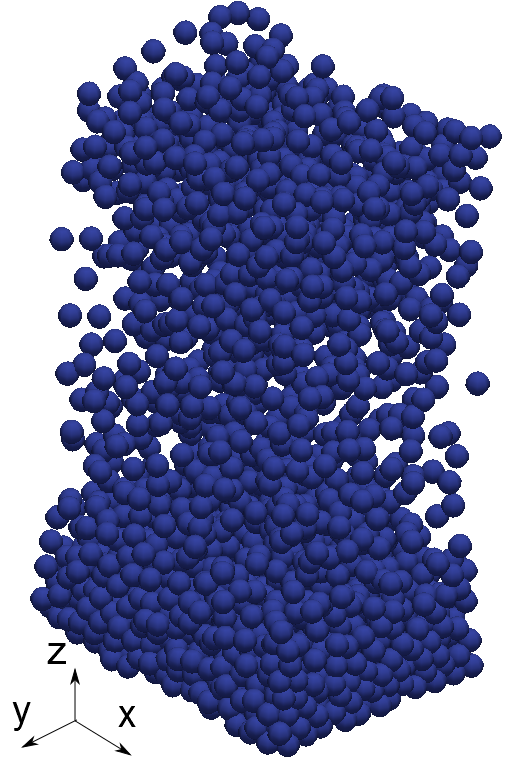
\includegraphics[width=\textwidth]{chapters/figures/fill01.png}
	\end{subfigure}
	\begin{subfigure}[b]{0.25\textwidth}
		\centering
		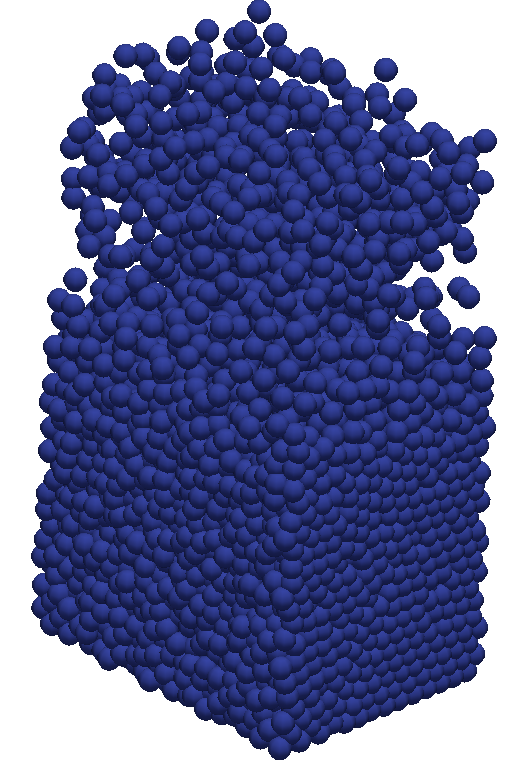
\includegraphics[width=\textwidth]{chapters/figures/fill02.png}
	\end{subfigure}
	\begin{subfigure}[b]{0.25\textwidth}
		\centering
		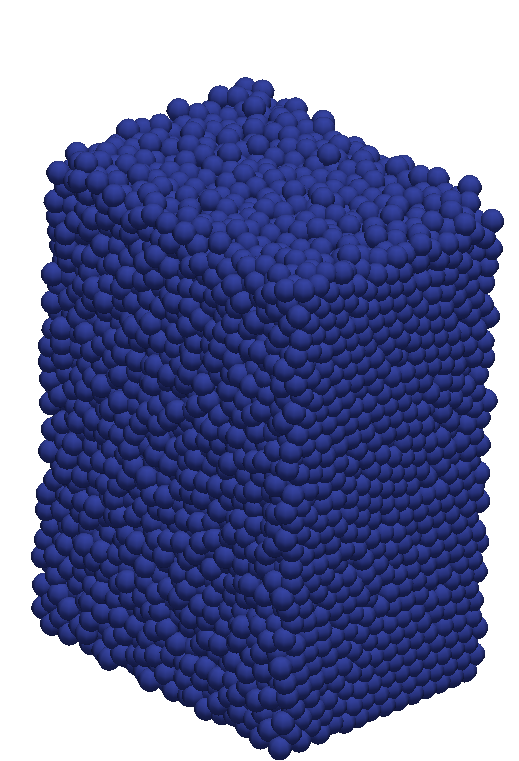
\includegraphics[width=\textwidth]{chapters/figures/fill03.png}
	\end{subfigure}
	\caption{Demonstrating the pouring process of $N = 10550$ pebbles into the control volume with at an early time (left), when it is nearly filled (middle) and after the pebbles have settled to negligible kinetic energy (right).}
\label{fig:fill01}
\end{figure}

In the end, a simpler pack-relax method was used instead. In this method $N$ particles are inserted into the volume such that we have precisely the packing fraction we desire (in this case, $\phi = 64\%$ so $N = 11000$). The pebbles are placed at random into the volume and are allowed to artificially overlap -- often by a great deal ($\delta \sim R_p$). The overlap they experience would normally cause such an enormous force (integrating into an enormous velocity) that the pebbles would all explode out of the bed at the first step in time integration. We avoid such a catostrophic scenario with a relaxation scheme where we truncate the displacement of any pebble per timestep that is integrated from the force. The truncated displacement is very small and allows the pebbles to slowly move away from each other and into a static equilibirum as the artifical overlap is reduced. Once the pebble bed comes to rest, we remove the relaxation (limiting displacement command) and allow standard integration of contact forces with the velocity-Verlet algorithm (see \cref{sec:velocity-verlet}). The pack-relax scheme allowed for obtaining desireable, highly repeatable packing fractions for all pebble beds. Once the pebble bed was packed into an initial condition, the simulation state was saved and used as a starting point for the numerous `crushed' cases to be described later.

In this first study, we model pebble crushing without considering why the particular pebble should be cracking. In the model we randomly select pebbles from the ensemble, regardless of forces acting upon the pebble, and delete them entirely from the system. When a pebble is removed, the neighboring pebbles react due to the imbalance of forces, and the bed settles into a new configuration. We differentiated the failed beds by their percentage of failed pebbles: $\eta = $ number of failed pebbles per original ensemble size. For the baseline case and for beds after failing, we apply the heating routine described next.

To simulate the conditions of a solid breeder in a fusion reactor, where the heat is removed from the pebble bed via contact to the containing structure, we assigned a constant temperature of $T_\text{c}$ to the vertical walls. Nuclear heating of the pebbles is simulated through a constant source term on each pebble. A representative heating rate of $Q_s = q_p'''V_p$, where  $q_p'''= 8$ MW/m$^3$. The heating cycle runs until a thermal steady state is reached. Based on a measurement of the total thermal energy of the bed, $E_T =\sum_i^N m_iC_i T_i$, steady-state is determined as $\dt{E_T} = 0$ within a specified tolerance. Once at steady state, we analyzed thermal and mechanical characteristics of the pebble bed: effective thermal conductivity, average coordination number, temperature profiles in the bed, and inter-particle contact forces. 

Based on the boundary conditions to our system, we establish heat transfer that is symmetric and one-dimensional in the $x$-direction from $x=0$ to the walls at $\frac{x}{d_p} = \pm 10$. As we will show, the pebble bed has very little variation of forces and temperatures in the $y$-direction due to the periodic boundary condition at the edges of the domain. Gravity effects are minor in the overall heat transfer and induce only a slight $z$-dependency to the results. We take advantage of this nature of our pebble bed to find the effective conductivity from an analytic, one-dimensional test case.
%~~~~~~~~~~~~~~~~~~~~~~~~~~~~~~~~~~~~~~~~~~~~~~~~~~~~~~~~~~~~~~~~~~~~~~





%~~~~~~~~~~~~~~~~~~~~~~~~~~~~~~~~~~~~~~~~~~~~~~~~~~~~~~~~~~~~~~~~~~~~~~
\subsection{Effective Thermal Conductivity from Analytic Analogy}
Assuming a one-dimensional pebble bed, to find an effective conductivity, we step back into a continuum mechanics formulation where the pebble bed can be represented as a slab of solid material. We can analytically solve for the temperature equation in a slab with heat generation, symmetry about the centerline, and a constant boundary temperature condition.

At steady-state, the temperature of a material with constant temperature boundary conditions ($T(L) = T_s$), constant thermal conductivity ($k_\text{eff}$), and nuclear heating ($q'''$) obeys the following equation

\begin{equation}\label{eq:continuum-heateqn}
	0 = \frac{\mathrm{d}^2T}{\mathrm{d}x^2} + \frac{q'''}{k_\text{eff}}
\end{equation}

We introduce a non-dimensional temperature
\begin{equation}
	\theta = \frac{T(x) - T_s}{T_0 - T_s}
\end{equation}
where $T_0$ is the temperature at the centerline of this slab (a value we will find momentarily). The length is non-dimensionalized as
\begin{equation}
	x^* = \frac{x}{L}
\end{equation}

Thus we can re-write Eq.~\ref{eq:continuum-heateqn} as
\begin{equation}\label{eq:continuum-heateqn-nondim}
	0 = \frac{\mathrm{d}^2\theta}{\mathrm{d}x^{*2}} + G
\end{equation}
where
\begin{equation}
	G = \frac{q'''L^2}{k_\text{eff}(T_0 - T_s)}
\end{equation}

In the non-dimensionalized form, the solution is revealed to be purely geometric,
\begin{equation}\label{eq:continuum-temperature-nondim}
	\theta = 1-x^{*2}
\end{equation}. 
as $T_0  - T_s = \frac{q'''L^2}{2k_\text{eff}}$. We will use the non-dimensional temperature solution of Eq.~\ref{eq:continuum-temperature-nondim} to prove our one-dimensional assumption of heat transfer is justified for the pebble beds.

We note that in this continuum mechanics formulation, we are assuming that the nuclear source, $q'''$ term is applied evenly over the entire volume. In our DEM formulation, our source term applies to a single pebble. To find the effective thermal conductivity of our `slab' of pebble bed, we must reconcile this discrepency. This is accomplished with the exchange of
\begin{equation}\label{eq:q-source-translation}
	q''' = \frac{Q_\text{tot}}{V_\text{tot}} = \frac{Q_sN}{H\cdot L\cdot W\cdot d_p^2}
\end{equation}
where the pebble bed volume is given by the height, $H$, width, $W$, and length, $L$, and $Q_s$ is the source term on each pebble in the DEM ensemble. 

From the solution of Eq.~\ref{eq:continuum-heateqn-nondim}, we find the effective conductivity to be
\begin{equation}
	k_\text{eff} = \frac{q''' L^2}{2(T_0-T_s)}
\end{equation}
and when we replace the heat generation term with Eq.~\ref{eq:q-source-translation}, and use the bed dimensions as given in \cref{sec:dem-setup}, this is written as
\begin{equation}\label{eq:dem-effecitve-conductivity-formula}
	k_\text{eff} = \frac{Q_sN}{180(T_0-T_s)d_p}
\end{equation}

We will use this formulation of Eq.~\ref{eq:dem-effecitve-conductivity-formula} to analyze and compare the pebble beds of this study.
% \begin{figure}[htbp]
% 	\centering
% 	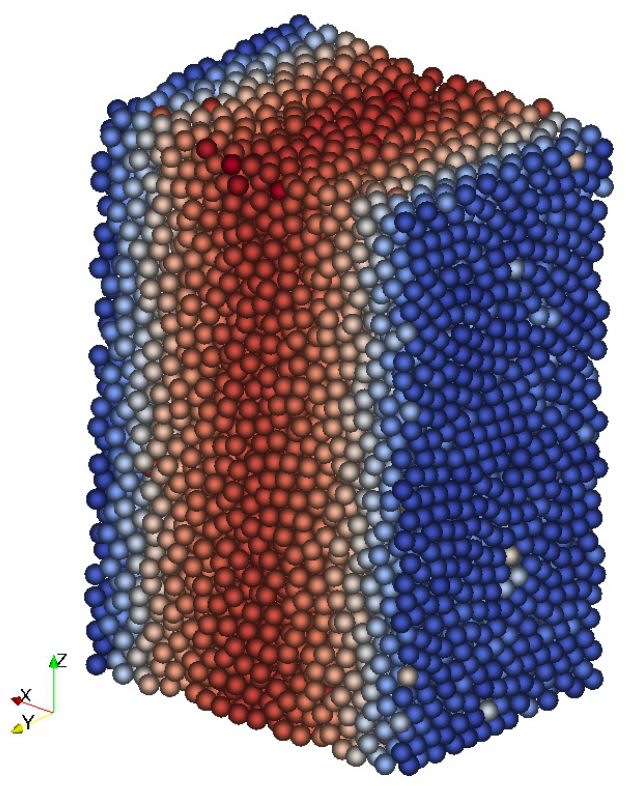
\includegraphics[trim=1cm 8cm 3cm 4cm, width=0.5\textwidth]{chapters/figures/pebbleBedTemperature}
% 	\caption{Temperature distribution of pebbles in the $10\%$ failed bed. At the end of steady-state heating, a one-dimensional profile is evident in all pebble beds studied here. The pebbles are receiving nuclear heating. Cooling proceeds through the pebbles in contact with the walls in the $x$-direction. [color online]}
% \label{fig:pebbleBedTemperature}
% \end{figure}

% \begin{figure}[htbp]
% 	\centering
% 	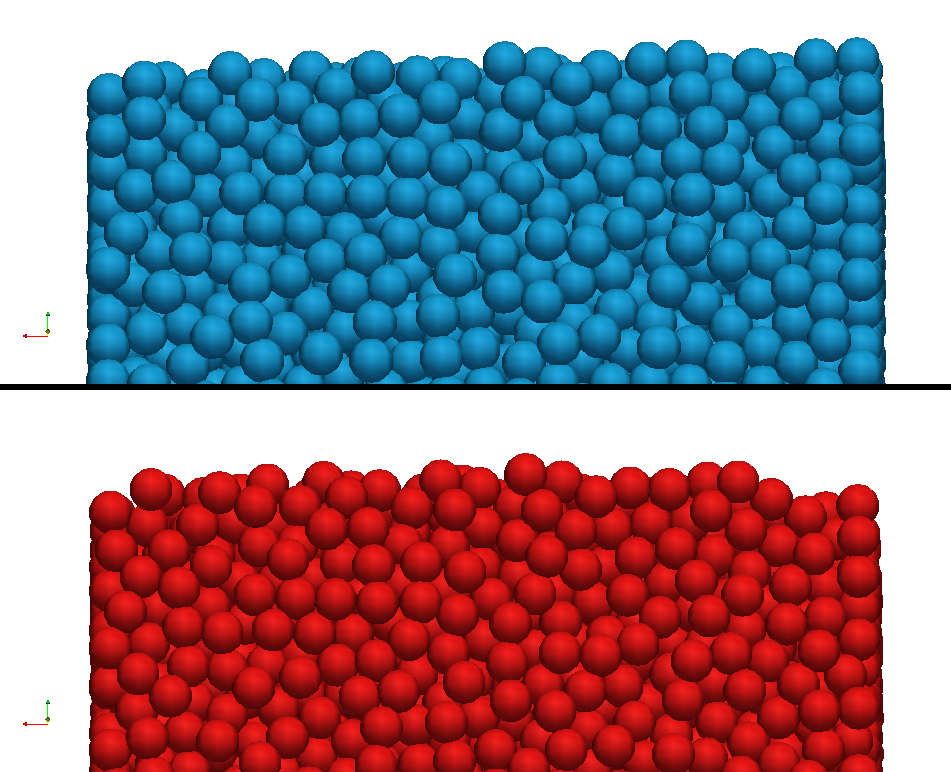
\includegraphics[width=0.5\textwidth]{chapters/figures/settlingStudy}
% 	\caption{Demonstrating the dynamic resettling from an example study done on location bias to pebble failure. The top image had the pebbles near the left wall biased to fail. The bottom image had a bias for the pebbles near both walls to fail. The lines are drawn as an aid to the eye.}
% \label{fig:settlingStudy}
% \end{figure}


\subsection{Results}
The aim of this study was both to discover the impact of pebble failure on thermomechanical properties as well as determine the impact as a function of the number of failed pebbles. To satisfy the latter, we created beds with $\eta = 1\%$, $3\%$, $5\%$, $10\%$, and $15\%$ of pebbles failed. 

We plot Eq.~\ref{eq:continuum-temperature-nondim} against the non-dimensionalized temperature profiles coming from the steady-state DEM simulation in Fig.~\ref{fig:tempProfile}. We find that all our models had a nearly perfect match to a one-dimensional prediction, validating the calculation of effective thermal conductivity in this study. Furthmore, the profiles adhering to the one-dimensional curve also allows us to find the effective conductivity of each bed from applying Eq.~\ref{eq:dem-effecitve-conductivity-formula}, which was derived from the one-dimensional assumption.

One concern we had for pebble crushing, was the phenomenon of `jamming' during resettling that would possibly leave pebbles isolated from their neighbors (apart from those they are resting upon). Jamming can happen when a bridge of pebbles have a balance for forces without strong or any contact to a pebble below them. The pebble under the bridge then only has light contact with the pebbles upon which it is resting. Such an isolated pebble would have no strong pathway for heat transfer and heat up much higher than that of its neighbors. Evidence of pebble isolation is apparent in hot individual pebbles above the grouped curve in Fig.~\ref{fig:temp-scatters}. 

\begin{figure}[htbp]
	\centering
	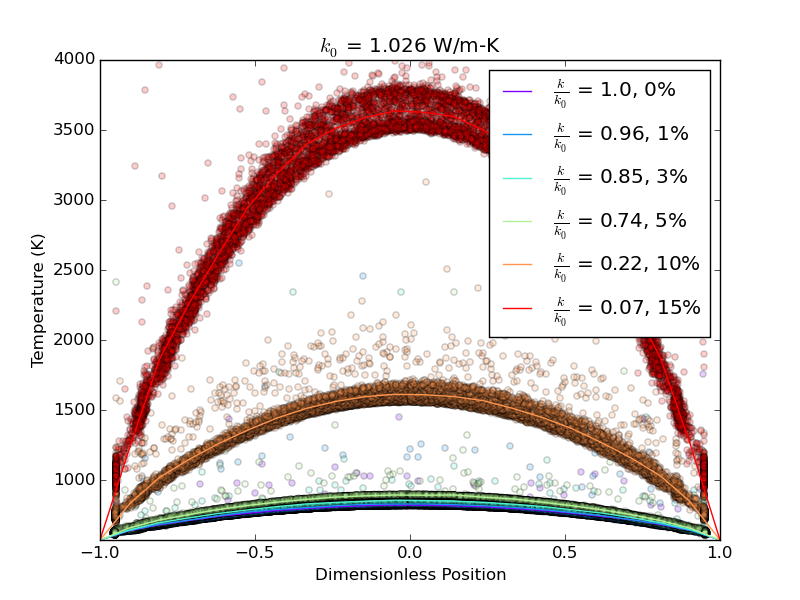
\includegraphics[width=0.65\textwidth]{chapters/figures/dem-evap-0-15-scatter-keff.png}
	\caption{The nondimensional temperature profiles for each test case follow the theoretical shape of a one-dimensional, constant $k$, continuum solution.}
\label{fig:tempProfile}
\end{figure}

The individual hot pebbles in Fig.~\ref{fig:temp-scatters} are also indicative of the shortcomings of the discrete element method for modeling solid breeders in fusion reactors. The flowing purge gas in actual solid breeders would likely not permit such thermal isolation of pebbles. Even if a pebble had no physical contact with neighboring ones, it would still transport energy via conduction and advection of the helium gas. This will be addressed again and in more detail in \cref{sec:cfd-dem-effective-conductivity}.

In order to calculate an effective conductivity of the pebble bed, we must find an average temperature profile through the bed to compare with Eq.~\ref{eq:continuum-temperature-nondim} and thus employ Eq.~\ref{eq:dem-effecitve-conductivity-formula}. We compare steady-state temperature profiles in the test beds against the one-dimensional, non-dimensional temperature profile. Average values of the bed, along the $x$ direction, are generated via averaging temperatures in bins. We create volumes slices of width $\Delta x$ that extend through the limits of the $y$- and $z$-directions. We then find the $n$ pebbles residing in the slices and take the mean value of their temperatures, 
\begin{equation}
	\langle T\rangle = \frac{1}{n}\sum_{i}^n T_i 	
\end{equation}
Using the volume slices, we also find the average coordination number, 
\begin{equation}
	\langle Z \rangle = \frac{1}{n}\sum_{i}^n Z_i
\end{equation}
normalized average contact force, 
\begin{equation}
	\langle F^* \rangle=\left[\langle F \rangle/\langle F_{bl} \rangle_\text{max}\right]^{1/3}
\end{equation}
and the normalized average temperature difference between pebbles in the slice,
\begin{equation}
	 \langle \Delta T_{ij} \rangle / (T_0 - T_s)_\text{bl}
\end{equation}


% \begin{figure}[htbp]
% 	\centering
% 	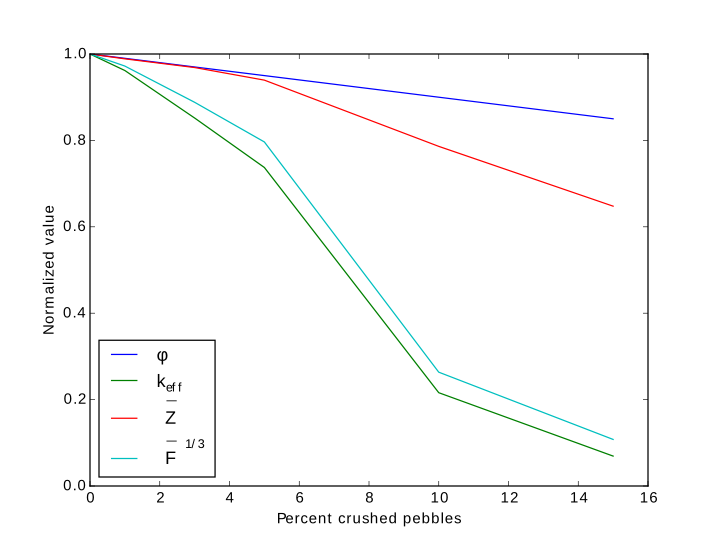
\includegraphics[width=0.65\textwidth]{chapters/figures/kEff_packingFraction}
% 	\caption{The normalized effective thermal conductivity (solid line) follows an exponential decay relationship with amount of failed pebbles. The normalized packing fraction (dashed line), compared to thermal conductivity, is relatively constant and is more closely fit to a linear reduction.}
% \label{fig:packingFraction}
% \end{figure}

% \begin{figure}[htbp]
% 	\centering
% 	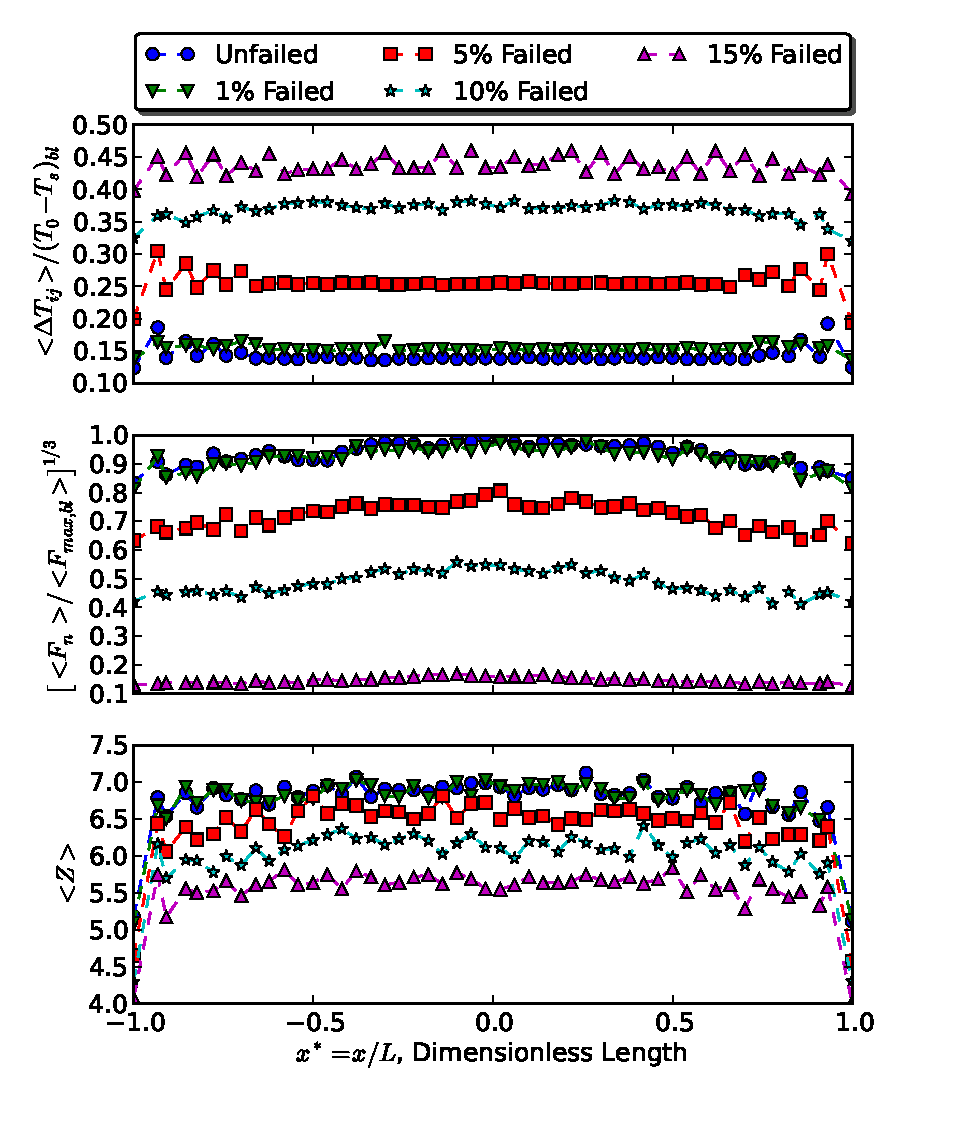
\includegraphics[width=0.75\textwidth]{chapters/figures/z_f_deltaT_subPlots}
% 	\caption{Average temperature differences between neighboring pebbles (top), contact forces (middle) and coordination numbers (bottom). The profiles of average coordination number and contact forces in the bed decrease in value with increasing pebble failure. Fewer and weaker contacts will reduce the possible paths of heat transfer from a pebble and this results in higher average temperatures between neighbors.}
% \label{fig:coordProfiles}
% \end{figure}


The effective thermal conductivity is found for all of our pebble beds, via Eq.~\ref{eq:dem-effecitve-conductivity-formula}, then normalized against the conductivity of the baseline ensemble ($k^* = k/k_\text{0}$). Figure~\ref{fig:packingFraction} shows the decreasing ETC with pebble failure. When $15\%$ of the pebbles are crushed in a pebble bed, the ETC has fallen all the way to only $k^*=0.07$. This large reduction is especially important in light of the already poor thermal management of virgin pebble beds that, even in helium environments, have been experimentally measured at only approximately 1~W/m-K (see, { e.g.}, Refs.~\cite{Reimann:2002mi, Piazza2002}). To find the cause of decrease in conductivity we make use of the inter-particle information provided by DEM tools instead of comparing macroscopic properties of packing fraction or external pressure.

In Eq.~\ref{eq:thermoFirstLaw} of \cref{sec:dem-heat-transfer}, we see that at steady-state, the energy input by nuclear heating must be balanced by the transport of heat out of a pebble into its neighbors. Inter-particle heat transfer is dictated by the number of neighboring contacts, temperature difference between pebbles, and the thermal conductance, $H_{c}$, through the contact area. The thermal conductance (see Eq.~\ref{eq:dem-conductance}) is itself a function purely of material properties  (which are essentially constant here) and the force at the contact, going as $H_{c} \propto F_{n,ij}^{1/3}$. Thus, we write the net heat out of a pebble at steady state as a function of the three variables,

\begin{equation}
	Q_\text{net} =f( Z, F_n^{1/3}, \Delta T)
\end{equation}



\begin{figure}[h!]
	\centering
	\begin{subfigure}[b]{0.45\textwidth}
		\centering
		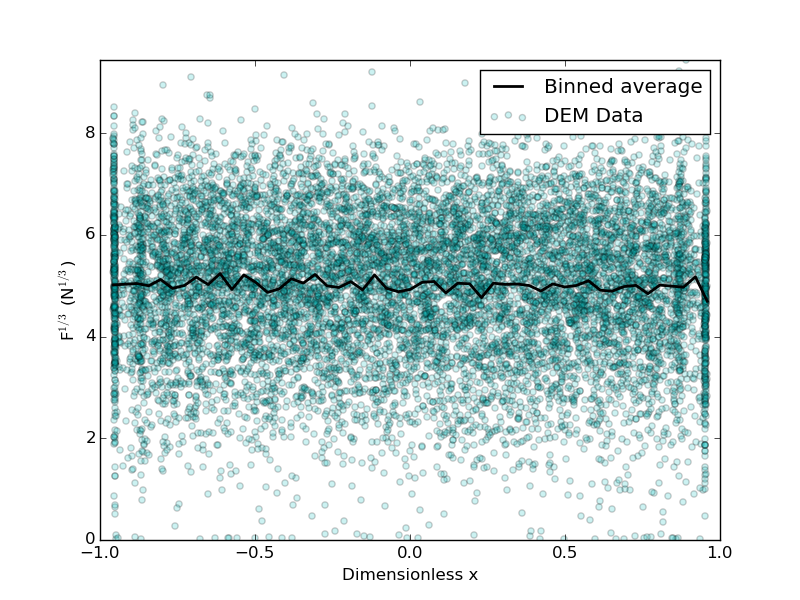
\includegraphics[width=\textwidth]{chapters/figures/heating_dte-02/0/dump/force-profile.png}
		\caption{Baseline pebble bed (0\% crushed)}
	\end{subfigure}
	\begin{subfigure}[b]{0.45\textwidth}
		\centering
		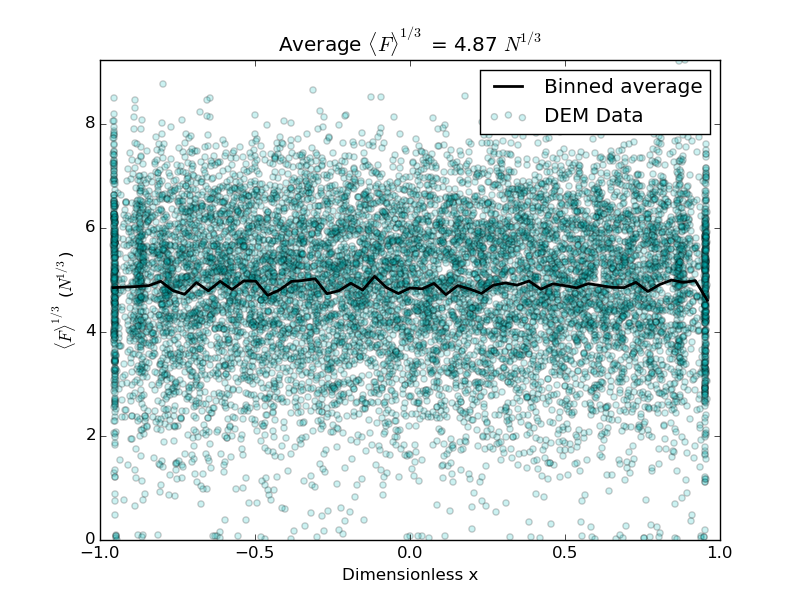
\includegraphics[width=\textwidth]{chapters/figures/heating_dte-02/1/dump/force-profile.png}
		\caption{1\% crushed}
	\end{subfigure}
	
	\begin{subfigure}[b]{0.45\textwidth}
		\centering
		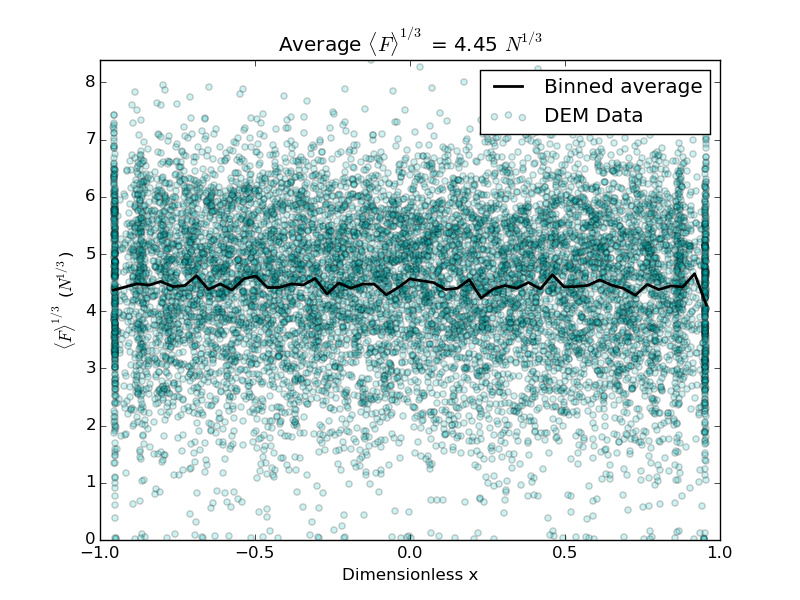
\includegraphics[width=\textwidth]{chapters/figures/heating_dte-02/3/dump/force-profile.png}
		\caption{3\% crushed}
	\end{subfigure}
	\begin{subfigure}[b]{0.45\textwidth}
		\centering
		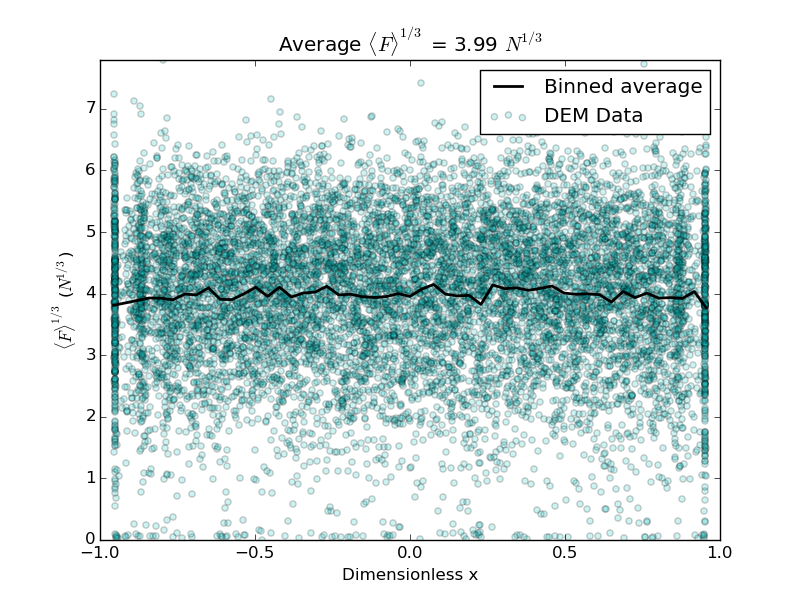
\includegraphics[width=\textwidth]{chapters/figures/heating_dte-02/5/dump/force-profile.png}
		\caption{5\% crushed}
	\end{subfigure}

	\begin{subfigure}[b]{0.45\textwidth}
		\centering
		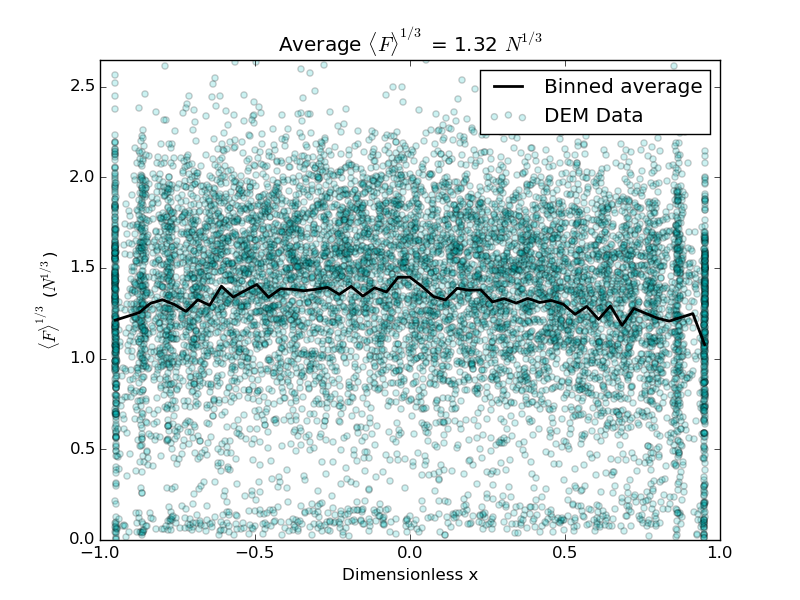
\includegraphics[width=\textwidth]{chapters/figures/heating_dte-02/10/dump/force-profile.png}
		\caption{10\% crushed}
	\end{subfigure}
	\begin{subfigure}[b]{0.45\textwidth}
		\centering
		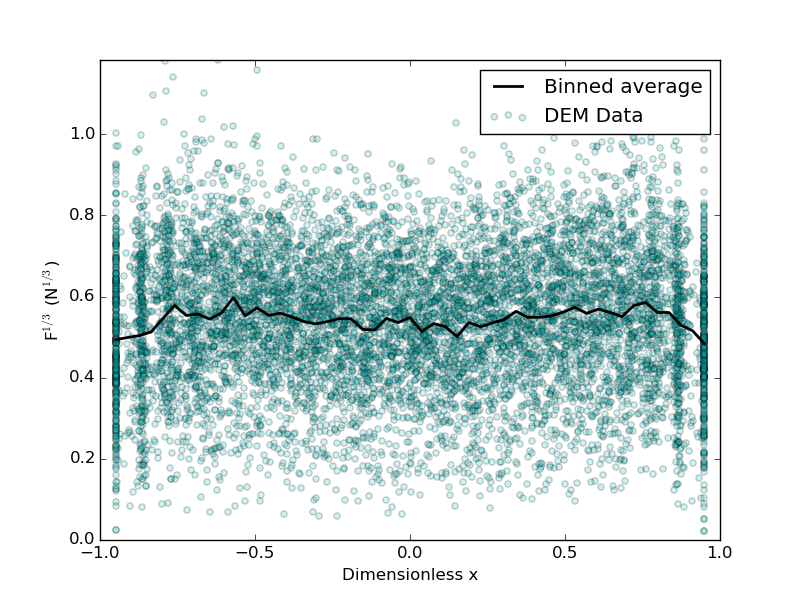
\includegraphics[width=\textwidth]{chapters/figures/heating_dte-02/15/dump/force-profile.png}
		\caption{15\% crushed}\label{fig:contact-forces-scatter-15percent}
	\end{subfigure}
	\caption{As pebble beds experience massive amounts of crushed pebbles (>5\%), the contact forces in the ensemble (after heating to steady-state) show dramatic reductions in value. Note the change of scale on the figures from the baseline case to the 15\% crushed case.}
\label{fig:contact-forces-scatter}
\end{figure}

The forces affecting $Q_\text{net}$ for the different levels of crushed pebbles are all plotted in Fig.~\ref{fig:contact-forces-scatter}. A dramatic reduction in the normal forces seen by pebbles after many of their neighbors are crushed and are removed from the system. From the baseline down to the 15\% failed case, the contact forces are reduced by about a factor of 10. 

Another feature of Fig.~\ref{fig:contact-forces-scatter} to point out is the change in distribution of average normal contact forces as the pebble beds experience crushed particles. For the well-packed beds of the baseline case up to the bed with 5\% crushed pebbles, the contact forces are relatively evenly distributed through the bed (i.e. the binned average line is relatively flat). However as substantial numbers of pebbles are induced to be crushed for the 10\% and 15\% beds, we see more of a dependence on location for contact force. This is based on the massive re-arrangement that happens in these beds. To demonstrate, we view the pebble bed of the 15\% crushed case in Fig.~\ref{fig:15percent-crushed-swelling}.

\begin{figure}[h!]
	\centering
	\begin{subfigure}[t]{0.45\textwidth}
		\centering
		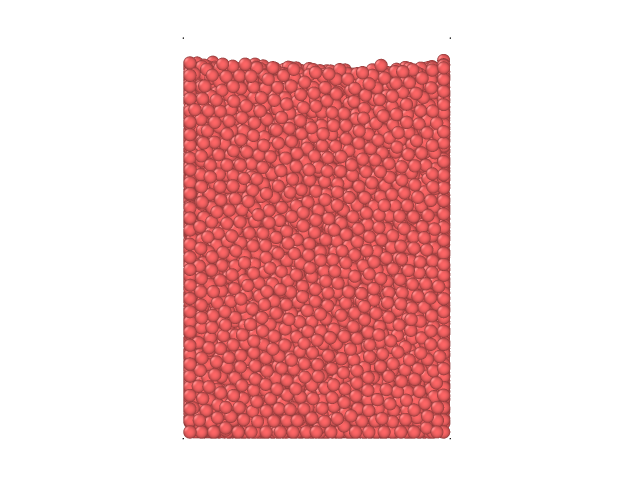
\includegraphics[width=\textwidth]{chapters/figures/heating_dte-02/15/0.15_pre_heat.png}
		\caption{Side-view of the pebble bed after resettling from the crushing event, before heating.}
	\end{subfigure}
	\begin{subfigure}[t]{0.45\textwidth}
		\centering
		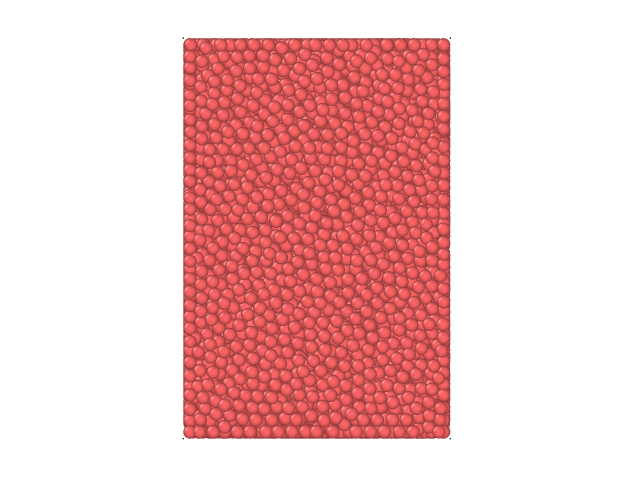
\includegraphics[width=\textwidth]{chapters/figures/heating_dte-02/15/0.15_post_heat.png}
		\caption{Side-view of the pebble bed after heating}
	\end{subfigure}
	\caption{In (a) we see the pebble bed after 15\% of the pebbles have been crushed (removed) and then after the heating cycle in (b). The gap formed after crushing is completely filled by swelling pebbles.}
\label{fig:15percent-crushed-swelling}
\end{figure}

After 15\% of the pebbles are removed from the system, a tremendous amount of resettling occurs and a large gap appears between the top wall and the top layer of pebbles. When heating is applied, the pebbles heat up very high until such time that they swell and press into each other with enough force to allow sufficient heat to conduct between them to balance the nuclear heating. Because of the resettling tending collapse toward the center, the residue of the resettling is apparent in the average normal contact forces of Fig.~\ref{fig:contact-forces-scatter-15percent}.





This reduction in force is joined by an increase in average neighbor temperatures which are 3 times higher for the bed with most failed pebbles when compared to the baseline. 

The average coordination number, shown in the bottom plot, decreases from a mid-line value of about 7.0 at the steady-state of the baseline case down to a mid-line value of 5.5 for the 15\% failed bed; a reduction of about 80\%. But this number doesn't compare with the large reduction in ETC which was $k_\text{eff}^*=0.30$. Clearly, there are fewer contacts in the pebble bed after failure but this alone does not account for the reduction in ETC.



The results shown in Fig.~\ref{fig:coordProfiles} demonstrate that the heat transfer through a pebble bed is simultaneously a function of the coordination number and inter-particle contact forces -- which are both reduced as pebbles in the bed fail -- as well as the temperature difference between pebbles at steady state -- which increases as pebbles in the ensemble fail. Interestingly, when a pebble bed has lower overall inter-particle contact forces fewer particles would be expected to break. This would imply that pebble breakage is self-dampening; as pebbles begin to break the ensemble quickly relaxes and avoids future pebble failure. So while we induced failure up to $\eta = 15\%$, such large values may not occur in real beds. 


